\subsection*{Tilpasning af træningsniveau}
Førend træningen kan påbegyndes tilpasses træningsniveauet den enkelte bruger. Tilpasning af træningsniveauet er inddelt i fire boundary. Disse håndteres af en samlet controller, hvilket fremgår af \autoref{fig:DesignTilpasning}.

\begin{figure} [H]
\centering
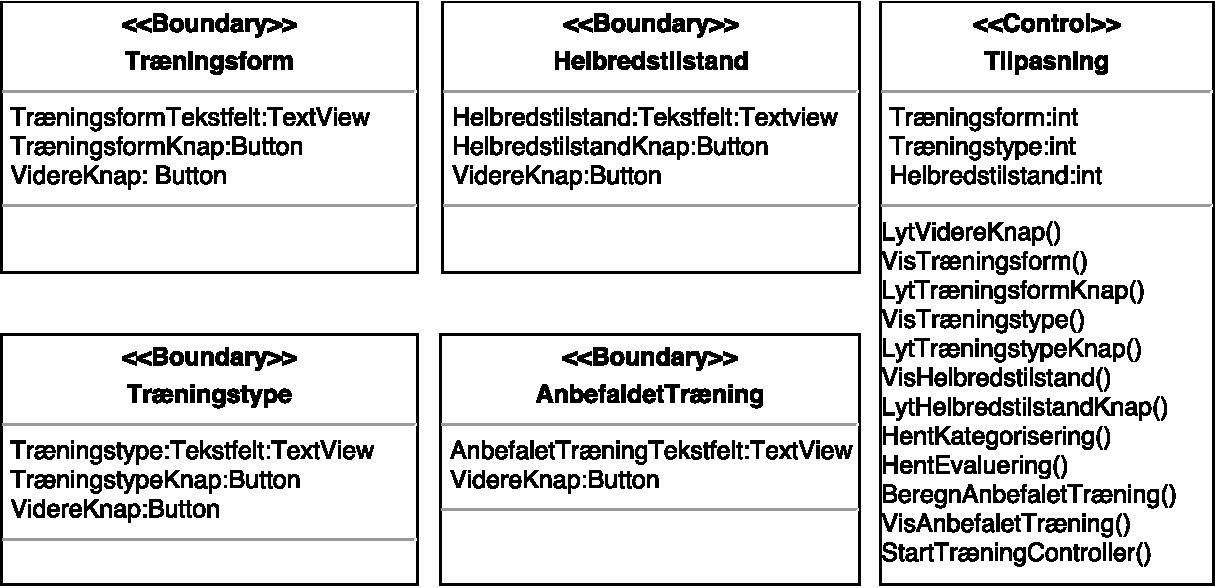
\includegraphics[width=0.9\textwidth]{figures/MVC/MVCTilpasning}
\caption{Designklasser for tilpasning af træningsniveau.}
\label{fig:DesignTilpasning}
\end{figure}

\noindent
Der er opstilles fire grænseflader for henholdsvis \textit{Træningsform}, \textit{Træningstype}, \textit{Helbredstilstand} og \textit{AnbefaldetTræning}. Dette er valgt, da det ønskes at gøre app’en overskuelig samt brugervenlig. Hertil skal brugeren foretage minimale valg på hver brugergrænseflade, således brugeren ikke eksponeres til for mange valg samt informationer. Til disse er der opstillet tekstfelter af typen textview og knapper af typen button.   

Den tilhørende controller, \textit{Tilpasning}, til de ovenstående boundarys lagrer den angivne træningsform, træningstype samt helbredstilstand, således disse senere kan benyttes til at beregne det passende træningsniveau. Der er opstillet vis, lyt, hent og beregn metoder til denne controller. 

Da det for brugeren skal være muligt at tilkoble kompatible enheder, forekommer endnu en controller. Denne skal håndterer kommunikation mellem systemet og kompatible måleenheder. Designklasse for kompatible måleenheder ses af \autoref{fig:kompatiblemåleenheder}.

\begin{figure} [H]
\centering
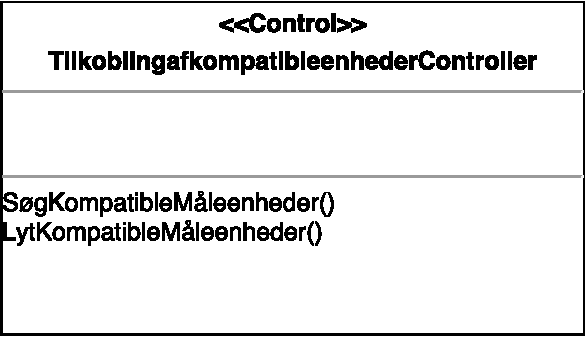
\includegraphics[width=0.6\textwidth]{figures/MVC/MVCKompMaale}
\caption{Designklasse for kompatible måleenheder.}
\label{fig:kompatiblemåleenheder}
\end{figure}

\noindent 
Controlleren, \textit{KompatibleEnheder}, tilgås ikke af brugeren, da det ønskes, at denne er en autonom funktion, der søger efter kompatible måleenheder førend en træning påbegyndes. Controlleren har en lyt og tilslut metode. 

Ud fra designklasserne er der udarbejdet et sekvensdiagram, hvilket fremgår af \autoref{fig:SEKTilpasning}. 

\begin{figure} [H]
\centering
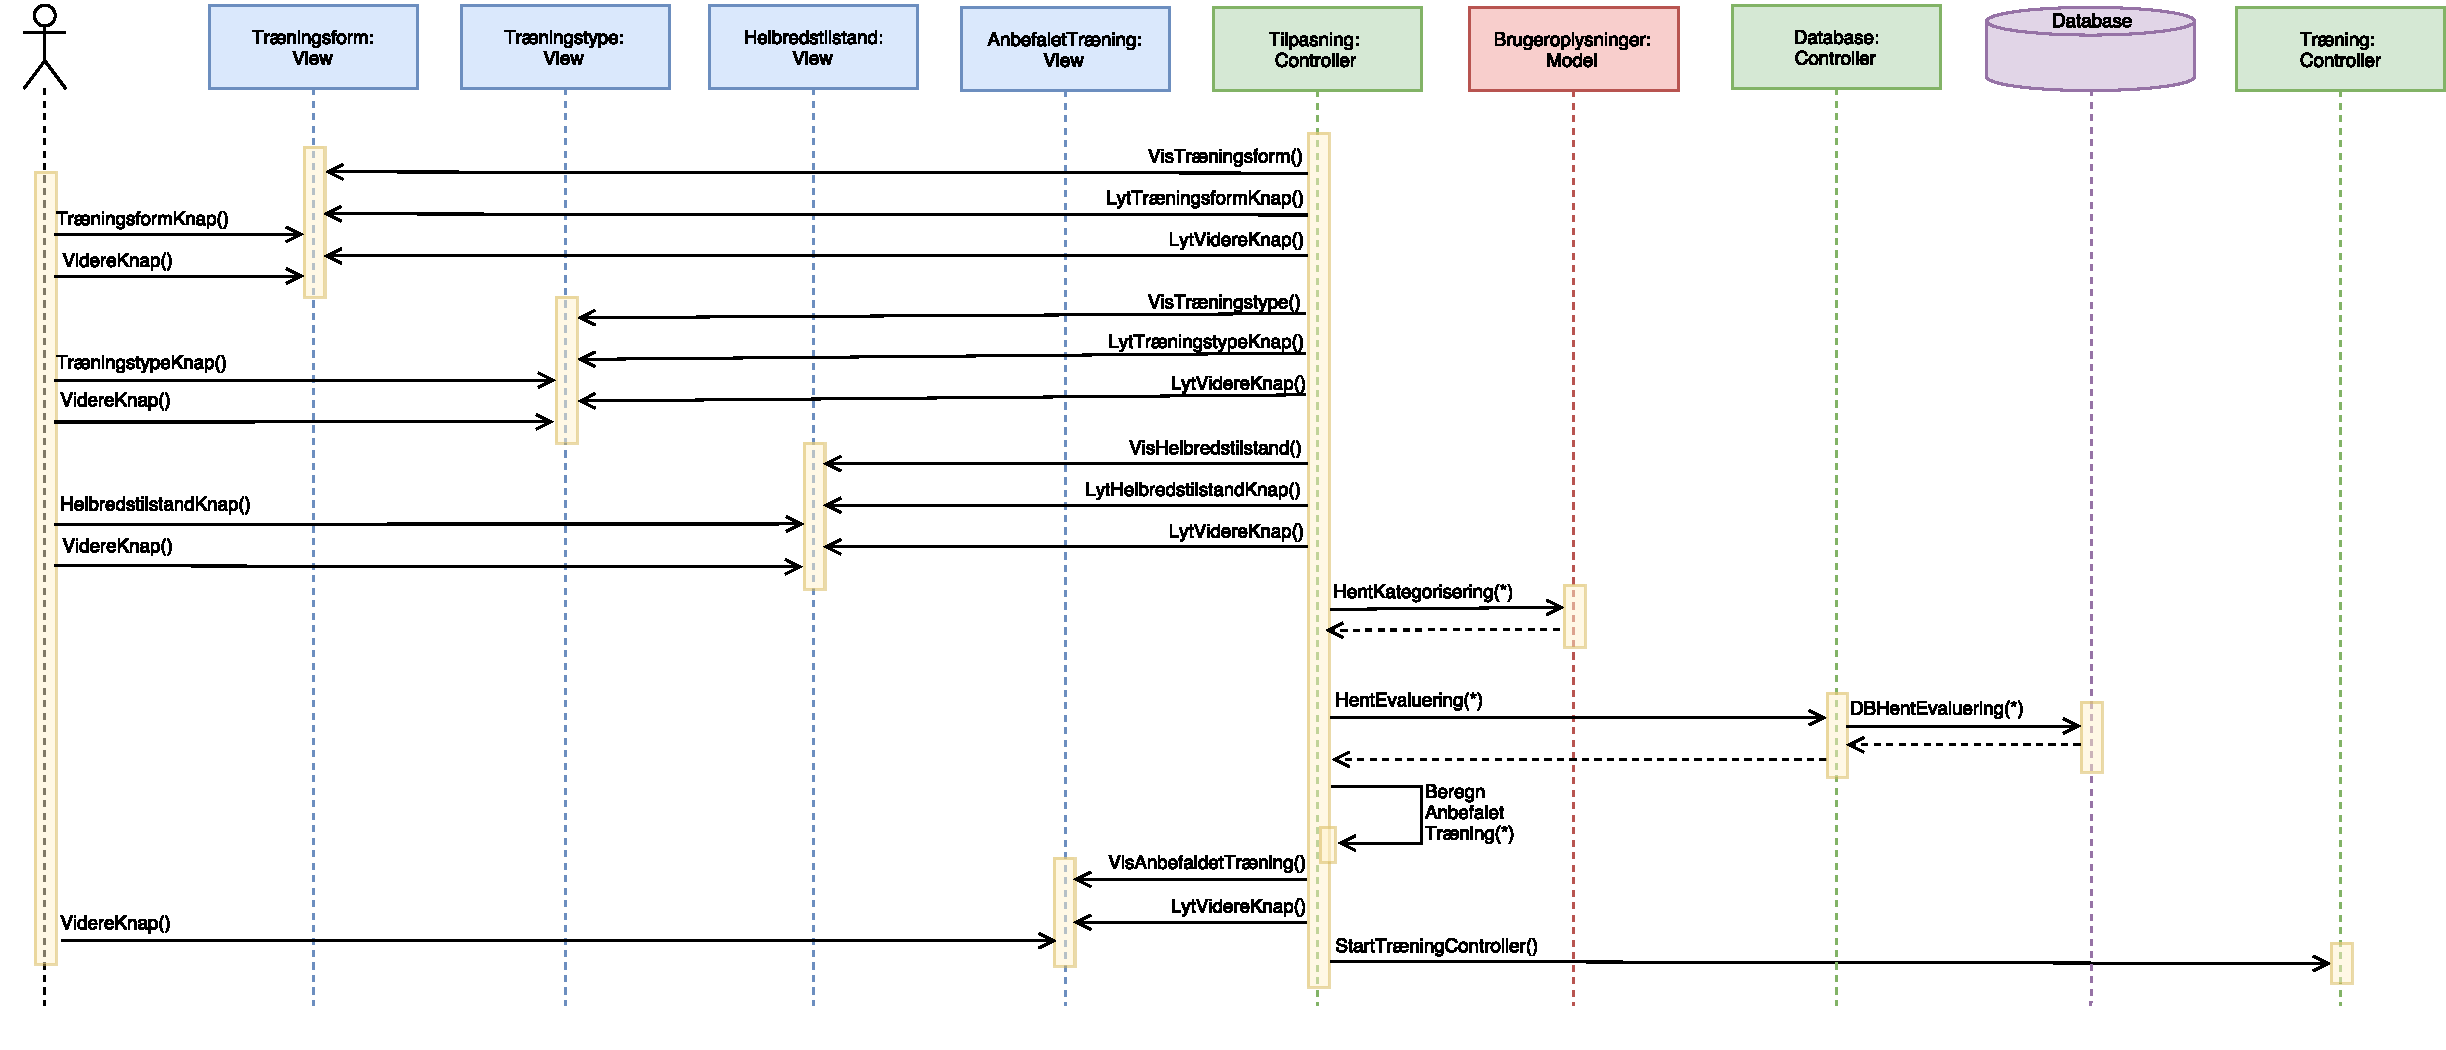
\includegraphics[width=1\textwidth]{figures/Sek/SEKTilpasning}
\caption{Sekvensdiagram for tilpasning af træningsniveau.}
\label{fig:SEKTilpasning}
\end{figure}

\noindent
Den første grænseflade som vises er \textit{Træningsform}. Denne grænseflade indeholder et tekstfelt, der beskriver, hvad brugeren skal angive. Dertil er der opstillet en TræningsformsKnap, hvor brugeren kan vælge mellem konditionstræning, styrketræning eller vejrtrækningsøvelser. Når der er angivet træningsform trykker brugeren på VidereKnap. Hvorefter controlleren, \textit{Tilpasning}, viser grænsefladen for valg af Træningstype. Brugeren skal her angive træningstype ud fra tre typer. Dette vil for eksempel ved konditionstræning være gå, løbe eller cykle. Brugeren angiver dette ved at trykke på VidereKnap, hvor efter controlleren viser grænsefladen for Helbredstilstand. Helbredstilstanden bekræftes ved at trykke på VidereKnap, herefter henter controlleren kategoriseringen i modellen for \textit{Brugeroplysninger}, denne er beskrevet i \autoref{sec:entity} og efterfølgende evaluering i \textit{Konditionstræning}. Controlleren lytter efter kompatible enheder fra den anden controller \textit{KompatibleEnheder}. Hvis \textit{KompatibleEnheder} controlleren prøver at tilslutte kompatible enheder, hvorefter denne sender besked til \textit{Tilspasning} controlleren om, hvorvidt tilslutning er lykkes eller mislykkes. Efterfølgende beregner controlleren anbefalet træningsniveau og viser dette på grænsefladen for \textit{AnbefaletTræning}. Brugeren kan herefter trykke på StartKnap, hvis denne trykkes på viser controlleren grænsefladen for \textit{Træning}. 




